\documentclass[aspectratio=169]{beamer}

\usetheme{Madrid}
\usecolortheme{default}
\setbeamertemplate{navigation symbols}{}
\usepackage{eso-pic}
\usepackage[brazil]{babel}
\shorthandoff{"}
\usepackage[T1]{fontenc}
\usepackage[utf8]{inputenc}
\usepackage{lmodern}
\usepackage{booktabs}
\usepackage{multirow}

\usepackage{tikz}
\usetikzlibrary{arrows.meta, positioning, shapes.geometric, shapes.symbols, fit, calc, backgrounds}
\usepackage{listings}
\usepackage{xcolor}
\usepackage{graphicx}

% --- Cores para listings ---
\definecolor{meuazul}{RGB}{0, 79, 151}
\definecolor{meucinza}{RGB}{80, 80, 80}
\definecolor{meuvermelhoescuro}{RGB}{180, 30, 30}
\definecolor{meuverde}{RGB}{30, 130, 60}
\definecolor{kotlinpurple}{RGB}{122, 44, 191}
\definecolor{kotlinorange}{RGB}{245, 130, 32}
\definecolor{codebg}{RGB}{245, 245, 250}
\definecolor{javabg}{RGB}{255, 248, 235}
\definecolor{codegreen}{RGB}{30, 130, 60}
\definecolor{codegray}{RGB}{128, 128, 128}
\definecolor{codeblue}{RGB}{0, 79, 151}
\setbeamercolor{structure}{fg=meuazul}

% --- Cores do diagrama TikZ ---
\definecolor{verde}{RGB}{76, 175, 80}
\definecolor{verdeescuro}{RGB}{46, 125, 50}
\definecolor{roxo}{RGB}{171, 71, 188}
\definecolor{ciano}{RGB}{0, 188, 212}
\definecolor{laranja}{RGB}{255, 152, 0}

% --- Estilos TikZ para o slide de Execução de programas ---
\tikzset{
  caixa/.style={
    draw, rounded corners=4pt, minimum width=1.8cm, minimum height=0.55cm,
    font=\tiny\bfseries, text centered, inner sep=3pt
  },
  caixaC/.style={caixa, fill=verde!80!black, text=white, draw=verde!60!black},
  caixaOS/.style={caixa, fill=roxo!80, text=white, draw=roxo!60!black},
  caixaKT/.style={caixa, fill=verde!80!black, text=white, draw=verde!60!black},
  caixaBC/.style={caixa, fill=ciano!80!black, text=white, draw=ciano!50!black, minimum width=2.4cm},
  caixaJVM/.style={caixa, fill=laranja!90, text=white, draw=laranja!70!black, minimum width=1.5cm},
  caixaPlat/.style={caixa, fill=roxo!80, text=white, draw=roxo!60!black, minimum width=1.5cm},
  seta/.style={-{Stealth[length=4pt]}, thick, gray!70},
}

% --- Estilo listings: Kotlin ---
\lstdefinelanguage{Kotlin}{
  keywords={fun, val, var, if, else, for, while, return, import, class, object, null, true, false, in, is, as, when, by, companion, override, data, sealed, interface, abstract, open, private, public, internal, protected, suspend, coroutine, out, in},
  keywordstyle=\bfseries\color{kotlinpurple},
  ndkeywords={String, Int, Boolean, Double, Float, Long, Array, List, ArrayList, Unit},
  ndkeywordstyle=\color{codeblue},
  sensitive=true,
  comment=[l]{//},
  morecomment=[s]{/*}{*/},
  commentstyle=\itshape\color{codegray},
  stringstyle=\color{codegreen},
  morestring=[b]",
}

% --- literate: suporte a caracteres acentuados dentro de lstlisting ---
\newcommand{\litlerate}{%
  literate=%
    {á}{{\'{a}}}1 {à}{{\`{a}}}1 {ã}{{\~{a}}}1 {â}{{\^{a}}}1
    {é}{{\'{e}}}1 {ê}{{\^{e}}}1
    {í}{{\'{i}}}1
    {ó}{{\'{o}}}1 {õ}{{\~{o}}}1 {ô}{{\^{o}}}1
    {ú}{{\'{u}}}1 {ü}{{\"u}}1
    {ç}{{\c{c}}}1
    {Á}{{\'{A}}}1 {À}{{\`{A}}}1 {Ã}{{\~{A}}}1
    {É}{{\'{E}}}1 {Ê}{{\^{E}}}1
    {Í}{{\'{I}}}1
    {Ó}{{\'{O}}}1 {Õ}{{\~{O}}}1
    {Ú}{{\'{U}}}1
    {Ç}{{\c{C}}}1
    {ã}{{\~{a}}}1%
}

% --- Estilo listings: Java personalizado ---
\lstdefinestyle{JavaStyle}{
  language=Java,
  keywordstyle=\bfseries\color{codeblue},
  commentstyle=\itshape\color{codegray},
  stringstyle=\color{codegreen},
  basicstyle=\ttfamily\scriptsize,
  backgroundcolor=\color{javabg},
  frame=single,
  rulecolor=\color{kotlinorange},
  numbers=none,
  breaklines=true,
  showstringspaces=false,
  tabsize=2,
  literate=
    {á}{{\'{a}}}1 {à}{{\`{a}}}1 {ã}{{\~{a}}}1 {â}{{\^{a}}}1
    {é}{{\'{e}}}1 {ê}{{\^{e}}}1
    {í}{{\'{i}}}1
    {ó}{{\'{o}}}1 {õ}{{\~{o}}}1 {ô}{{\^{o}}}1
    {ú}{{\'{u}}}1
    {ç}{{\c{c}}}1
    {Á}{{\'{A}}}1 {É}{{\'{E}}}1 {Í}{{\'{I}}}1 {Ó}{{\'{O}}}1 {Ú}{{\'{U}}}1
    {Ç}{{\c{C}}}1,
}

% --- Estilo listings: Kotlin personalizado ---
\lstdefinestyle{KotlinStyle}{
  language=Kotlin,
  basicstyle=\ttfamily\scriptsize,
  backgroundcolor=\color{codebg},
  frame=single,
  rulecolor=\color{kotlinpurple},
  numbers=none,
  breaklines=true,
  showstringspaces=false,
  tabsize=2,
  literate=
    {á}{{\'{a}}}1 {à}{{\`{a}}}1 {ã}{{\~{a}}}1 {â}{{\^{a}}}1
    {é}{{\'{e}}}1 {ê}{{\^{e}}}1
    {í}{{\'{i}}}1
    {ó}{{\'{o}}}1 {õ}{{\~{o}}}1 {ô}{{\^{o}}}1
    {ú}{{\'{u}}}1
    {ç}{{\c{c}}}1
    {Á}{{\'{A}}}1 {É}{{\'{E}}}1 {Í}{{\'{I}}}1 {Ó}{{\'{O}}}1 {Ú}{{\'{U}}}1
    {Ç}{{\c{C}}}1,
}

\title[Introdução ao Kotlin]{Introdução ao Kotlin}
\subtitle{Desenvolvimento de Software para Dispositivos Móveis}
\author{Prof. Me. Sergio Souza Novak — UniRV}
\titlegraphic{
\includegraphics[width=2cm]{logo.png}}

\begin{document}

% Slide de Título
\frame[plain]{\titlepage}

% -------------
% Sumário automático
% -------------
\begin{frame}{Sumário}
  \footnotesize
  \begin{columns}[T]
    \begin{column}{0.48\textwidth}
      \tableofcontents[sections={1-4}]
    \end{column}
    \begin{column}{0.48\textwidth}
      \tableofcontents[sections={5-8}]
    \end{column}
  \end{columns}
\end{frame}

% -----------------------------------------------
% Seção: O que é Kotlin?
% -----------------------------------------------
\section{O que é Kotlin?}

\begin{frame}{O que é Kotlin?}
  \begin{columns}[c]
    \begin{column}{0.62\textwidth}
      \begin{itemize}\small
        \item Linguagem de programação moderna, estaticamente tipada e de uso geral.
        \item Criada pela JetBrains em 2011.
        \item Tornou-se a linguagem oficial para desenvolvimento Android pelo Google em 2017.
        \item 100\% interoperável com Java.
        \item Código aberto (Open Source).
        \item Suporta desenvolvimento Android, Web (JS/Wasm), Desktop e Multiplataforma (KMP).
      \end{itemize}
    \end{column}

    \begin{column}{0.35\textwidth}
      \centering
      
\includegraphics[width=\textwidth]{images/kotlin_logo.png}
    \end{column}
  \end{columns}
\end{frame}

% -----------------------------------------------
% Seção: Características
% -----------------------------------------------
\section{Características da Linguagem}

\begin{frame}[fragile,shrink=5]{Características}

  \begin{columns}[T]

    % --- Coluna Esquerda: lista de características ---
    \begin{column}{0.43\textwidth}

      % 100% compatível com Java
      \begin{block}{\centering 100\% compatível com Java}
        \centering
        {\color{kotlinpurple}\textbf{\large Kotlin}} \quad {\color{kotlinorange}\textbf{\large Java}}
      \end{block}

      \vspace{0.2em}
      \begin{itemize}\footnotesize
        \item \textbf{Interoperável:} usa classes nativas do Java em Kotlin. {\tiny $\nearrow$}
        \item Orientada a objetos \textbf{e} funcional.
        \item Estaticamente tipada.
        \item Concisa.
        \item \textbf{Segura:} tratamento de nulos (Null Safety). {\tiny $\downarrow$}
      \end{itemize}
    \end{column}

    % --- Coluna Direita: exemplo de interoperabilidade ---
    \begin{column}{0.55\textwidth}
      {\footnotesize\textbf{Interoperabilidade — \texttt{ArrayList} Java em Kotlin:}}
      \vspace{0.1em}

\begin{lstlisting}[style=KotlinStyle]
import java.util.ArrayList

fun main(args: Array<String>) {
    val lista = ArrayList<String>() // lista Java
    lista.add("Sergio")
    lista.add("Leandro")
    for (item in lista) {
        System.out.println(item) // java
        println(item)            // kotlin
    }
}
\end{lstlisting}
    \end{column}

  \end{columns}

  % --- Parte inferior: comparativo Null Safety ---
  \noindent\rule{\textwidth}{0.4pt}
  {\footnotesize\textbf{Null Safety — Kotlin vs.\ Java:}}

  \begin{columns}[T]

    % Kotlin
    \begin{column}{0.49\textwidth}
      {\footnotesize\textcolor{kotlinpurple}{\textbf{Kotlin}}}
\begin{lstlisting}[style=KotlinStyle]
var valor: String? = null
println(valor.equals("Sergio"))
// Resultado: false
\end{lstlisting}
      {\tiny\textit{Kotlin lida com \texttt{String?} de forma segura, retornando \texttt{false}.}}
    \end{column}

    % Java
    \begin{column}{0.49\textwidth}
      {\footnotesize\textcolor{kotlinorange}{\textbf{Java}}}
\begin{lstlisting}[style=JavaStyle]
String valor = null;
System.out.println(valor.equals("Leandro"));
// java.lang.NullPointerException
\end{lstlisting}
      {\tiny\textit{Chamar método em \texttt{null} dispara \texttt{NullPointerException}.}}
    \end{column}

  \end{columns}

\end{frame}

% -----------------------------------------------
% Seção: Execução de programas
% -----------------------------------------------
\section{Execução de Programas}

\begin{frame}[t,fragile]{Execução de programas}

  \begin{columns}[T]

    %--- COLUNA ESQUERDA: Processo genérico (linguagem C) ---
    \begin{column}{0.47\textwidth}
      \begin{itemize}\footnotesize
        \item Processo para execução de um programa
        \begin{itemize}\scriptsize
          \item[$\circ$] Escrita
          \item[$\circ$] Compilação
          \item[$\circ$] Execução
        \end{itemize}
      \end{itemize}
      \begin{center}
      \begin{tikzpicture}[node distance=0.4cm and 0.6cm]
        \node[caixaC, minimum width=2.0cm] (progC) {Programa em C};

        \node[caixaKT, minimum width=2.1cm, below right=0.5cm and 0.4cm of progC] (ccwin)
          {\shortstack{Compilador C\\Windows}};
        \node[caixaKT, minimum width=2.1cm, below=0.3cm of ccwin] (cclin)
          {\shortstack{Compilador C\\Linux}};
        \node[caixaKT, minimum width=2.1cm, below=0.3cm of cclin] (ccmac)
          {\shortstack{Compilador C\\Mac}};

        \node[caixaOS, right=0.4cm of ccwin] (win) {Windows};
        \node[caixaOS, right=0.4cm of cclin] (lin) {Linux};
        \node[caixaOS, right=0.4cm of ccmac] (mac) {Mac};

        % Conexões ortogonais (|-) conforme imagem
        \draw[seta] (progC.south) |- (ccwin.west);
        \draw[seta] (progC.south) |- (cclin.west);
        \draw[seta] (progC.south) |- (ccmac.west);

        \draw[seta] (ccwin) -- (win);
        \draw[seta] (cclin) -- (lin);
        \draw[seta] (ccmac) -- (mac);
      \end{tikzpicture}
      \end{center}
    \end{column}

    %--- COLUNA DIREITA: Processo Kotlin/Java ---
    \begin{column}{0.51\textwidth}
      \begin{itemize}\footnotesize
        \item Processo para execução de um programa Kotlin/Java
        \begin{itemize}\scriptsize
          \item[$\circ$] Escrita
          \item[$\circ$] Compilação
          \item[$\circ$] Execução
        \end{itemize}
      \end{itemize}
      \begin{center}
      \begin{tikzpicture}[node distance=0.45cm and 0.8cm]
        \node[caixaKT] (kt)   {Kotlin (.kt)};
        \node[caixaKT, right=0.8cm of kt] (java) {Java (.java)};

        \node[caixaKT, minimum width=1.9cm, below=0.45cm of kt]
          (kotlinc) {\shortstack{Kotlinc\\(compilador)}};
        \node[caixaKT, minimum width=1.9cm, below=0.45cm of java]
          (javac)   {\shortstack{Javac\\(compilador)}};

        \node[caixaBC, below right=0.45cm and -0.65cm of kotlinc] (bc)
          {Byte code (.class)};

        \node[caixaJVM, below left=0.45cm and 0.05cm of bc]  (jvm1) {JVM};
        \node[caixaJVM, below=0.45cm of bc]                   (jvm2) {JVM};
        \node[caixaJVM, below right=0.45cm and 0.05cm of bc]  (jvm3) {JVM};

        \node[caixaPlat, below=0.35cm of jvm1] (plin) {Linux};
        \node[caixaPlat, below=0.35cm of jvm2] (pwin) {Windows};
        \node[caixaPlat, below=0.35cm of jvm3] (pmac) {Mac};

        \node[right=0.1cm of jvm3, font=\tiny, align=left]
          {\shortstack[l]{Java Virtual\\Machine}};

        \draw[seta] (kt)      -- (kotlinc);
        \draw[seta] (java)    -- (javac);
        \draw[seta] (kotlinc.south) |- (bc.north);
        \draw[seta] (javac.south)   |- (bc.north);
        \draw[seta] (bc.south) |- (jvm1.north);
        \draw[seta] (bc.south) -- (jvm2.north);
        \draw[seta] (bc.south) |- (jvm3.north);
        \draw[seta] (jvm1) -- (plin);
        \draw[seta] (jvm2) -- (pwin);
        \draw[seta] (jvm3) -- (pmac);
      \end{tikzpicture}
      \end{center}
    \end{column}

  \end{columns}

\end{frame}

% -----------------------------------------------
% Seção: Primeiro Hello World em Kotlin
% -----------------------------------------------
\section{Primeiro Hello World em Kotlin}

\subsection{Criando e Configurando o Projeto}

% Slide 1: Criando um Novo Projeto
\begin{frame}{Criando um Novo Projeto no IntelliJ IDEA}
  \begin{columns}[T]
    \begin{column}{0.4\textwidth}
      \vspace{1em}
      \begin{itemize}\small
        \item Abra o \textbf{IntelliJ IDEA}.
        \item Na tela inicial de boas-vindas, clique no botão \textbf{New Project} (\texttt{+}).
      \end{itemize}
    \end{column}
    \begin{column}{0.58\textwidth}
      \centering
      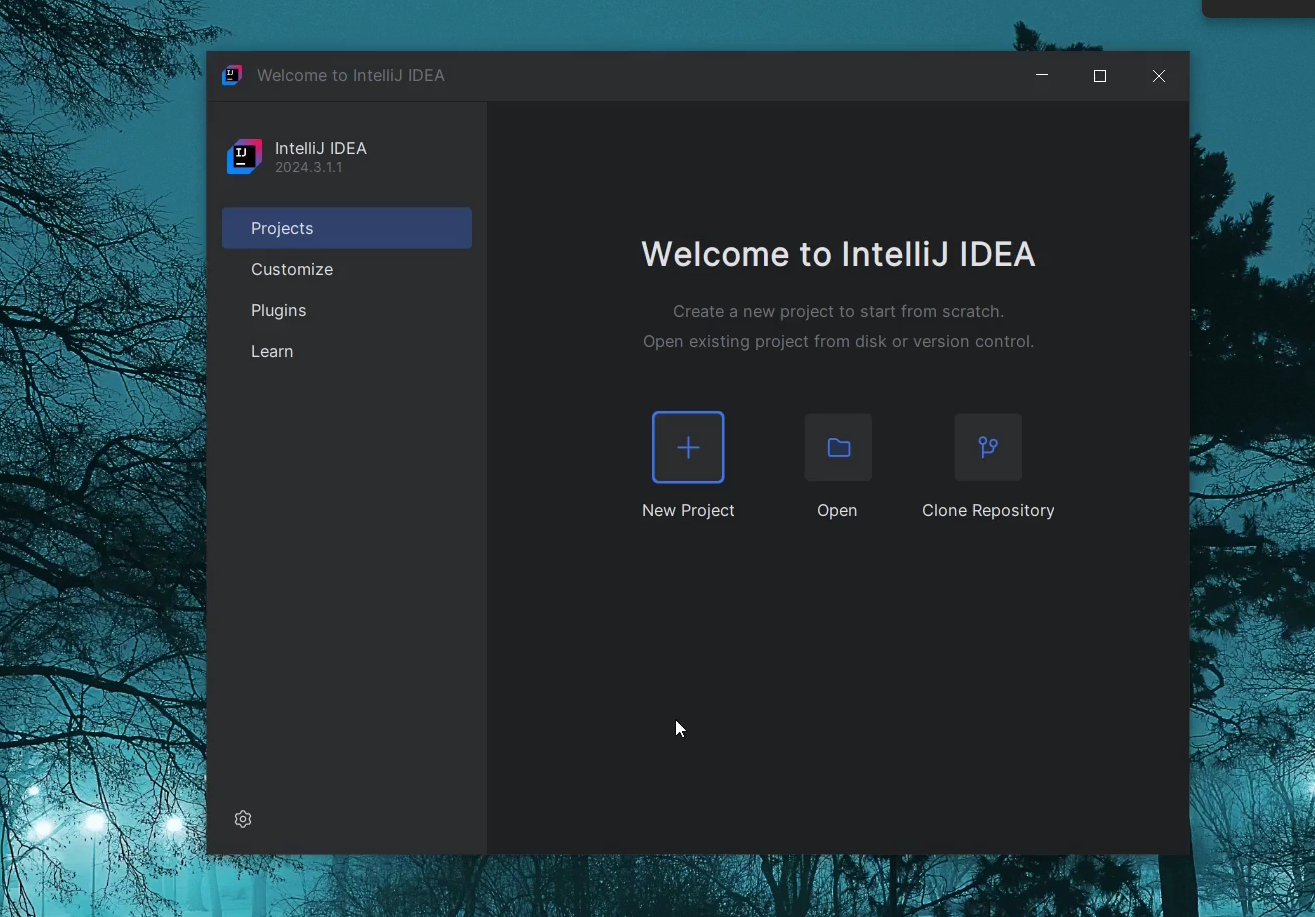
\includegraphics[width=\textwidth]{images/Captura de tela de 2026-07-31 09-58-03.png}
    \end{column}
  \end{columns}
\end{frame}

% Slide 2: Configurando o Projeto
\begin{frame}[shrink=10]{Configurando o Projeto Kotlin}
  \begin{columns}[T]
    \begin{column}{0.4\textwidth}
      \vspace{0.5em}
      \begin{itemize}\small
        \item Selecione \textbf{Kotlin} no painel esquerdo.
        \item Defina o nome do projeto (ex: \texttt{HelloWorld}).
        \item Escolha o local no disco.
        \item Selecione o \textbf{Build system} (IntelliJ ou Gradle) e a \textbf{JDK} desejada.
        \item Clique em \textbf{Create}.
      \end{itemize}
    \end{column}
    \begin{column}{0.58\textwidth}
      \centering
      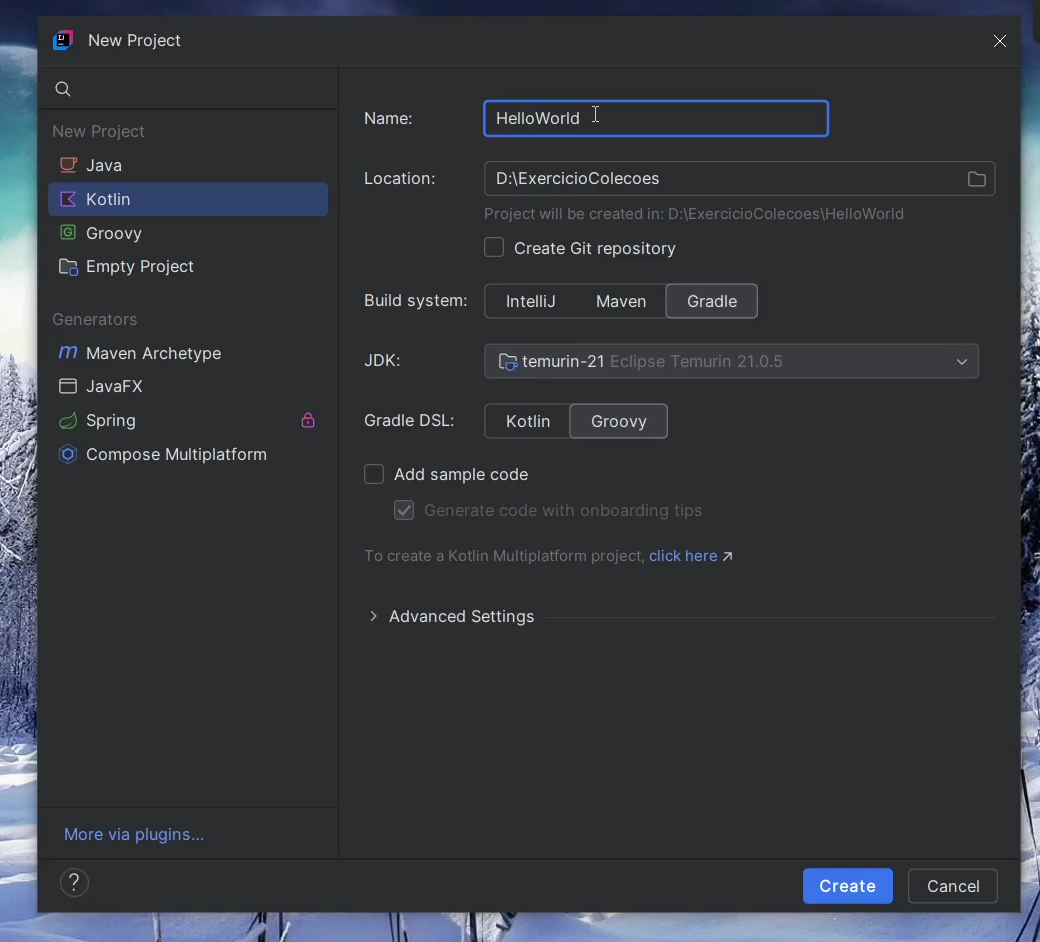
\includegraphics[width=\textwidth]{images/Captura de tela de 2026-07-31 09-59-11.png}
    \end{column}
  \end{columns}
\end{frame}

\subsection{Estrutura e Execução}

% Slide 3: Estrutura do Projeto e Código Main.kt
\begin{frame}{Estrutura do Projeto e Código Inicial}
  \begin{columns}[T]
    \begin{column}{0.42\textwidth}
      \vspace{0.5em}
      \begin{itemize}\small
        \item O arquivo principal é o \texttt{Main.kt} dentro da pasta \texttt{src}.
        \item A função principal \texttt{fun main()} é o ponto de entrada da aplicação.
        \item Utilize o ícone de reprodução verde ($\triangleright$) ao lado da linha para executar o código.
      \end{itemize}
    \end{column}
    \begin{column}{0.56\textwidth}
      \centering
      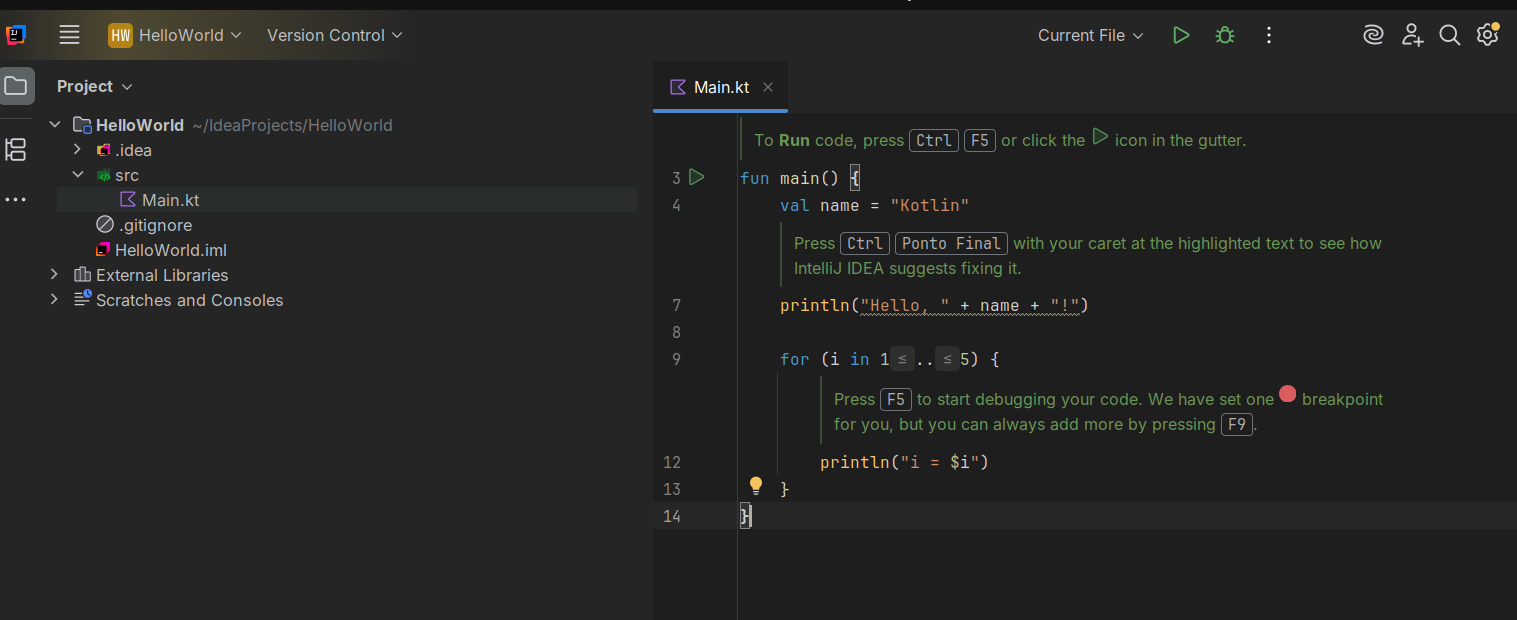
\includegraphics[width=\textwidth]{images/Captura de tela de 2026-07-31 10-05-10.png}
    \end{column}
  \end{columns}
\end{frame}

% Slide 4: Executando o Programa e Analisando a Saída
\begin{frame}{Executando e Analisando o Terminal de Saída}
  \begin{columns}[T]
    \begin{column}{0.42\textwidth}
      \vspace{1em}
      \begin{itemize}\small
        \item Ao executar, o painel \textbf{Run} é exibido na parte inferior.
        \item A saída do comando \texttt{println()} será impressa no console.
        \item O código de saída \texttt{exit code 0} indica execução com sucesso.
      \end{itemize}
    \end{column}
    \begin{column}{0.56\textwidth}
      \centering
      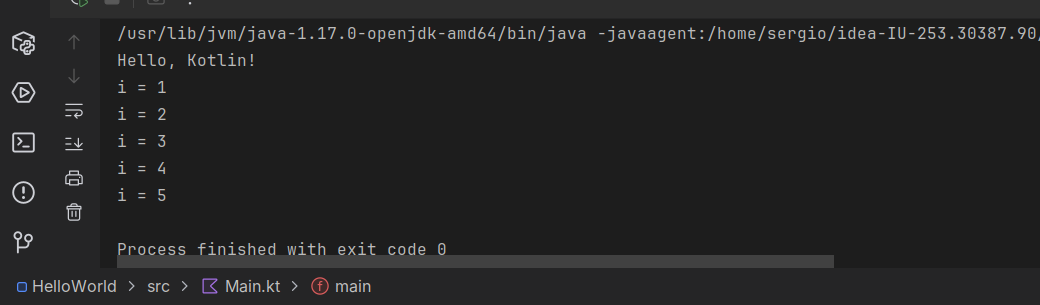
\includegraphics[width=\textwidth]{images/Captura de tela de 2026-07-31 10-06-00.png}
    \end{column}
  \end{columns}
\end{frame}

\subsection{Projetos Gradle e Pacotes}

% Slide 5: Projetos com Gradle (build.gradle.kts)
\begin{frame}{Estrutura com Gradle (\texttt{build.gradle.kts})}
  \begin{columns}[T]
    \begin{column}{0.42\textwidth}
      \vspace{0.5em}
      \begin{itemize}\small
        \item Em projetos Gradle, o arquivo \texttt{build.gradle.kts} define as configurações.
        \item Declara plugins (como \texttt{kotlin("jvm")}), repositórios e dependências.
        \item O código-fonte fica em \texttt{src/main/kotlin/}.
      \end{itemize}
    \end{column}
    \begin{column}{0.56\textwidth}
      \centering
      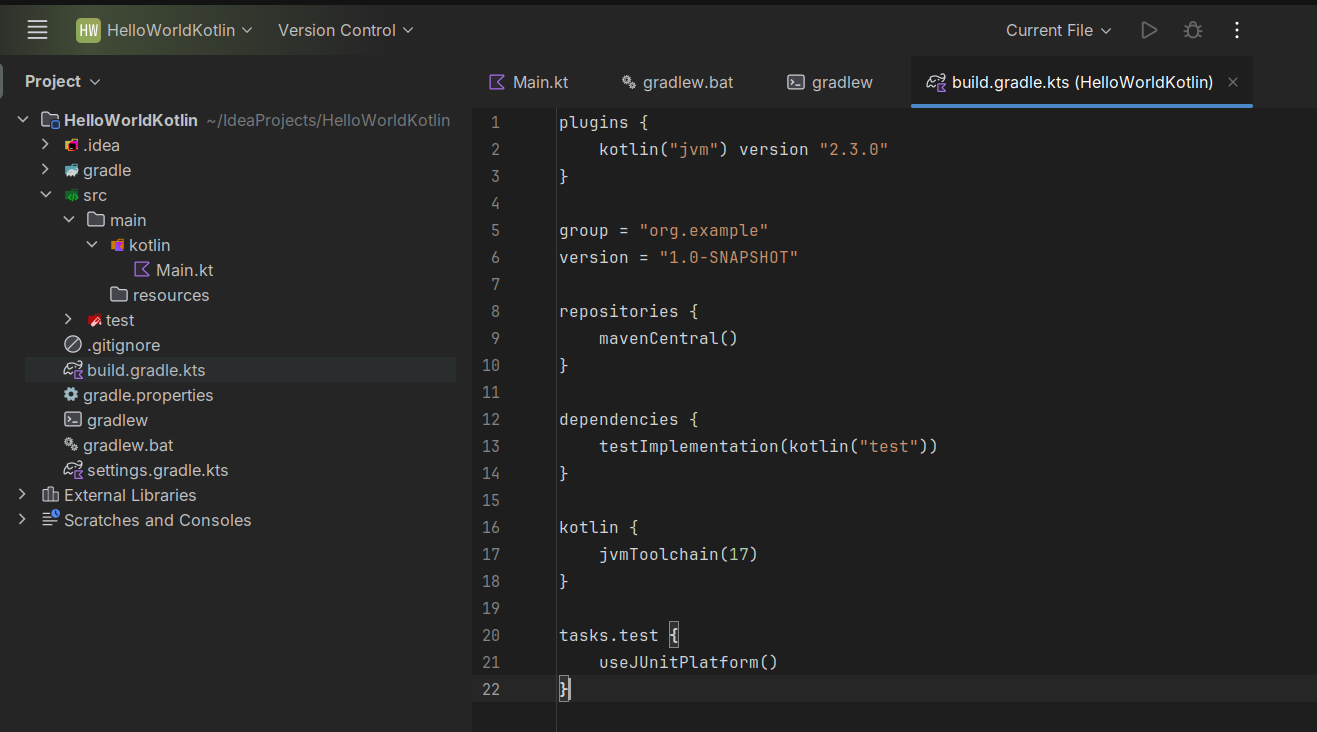
\includegraphics[width=\textwidth]{images/Captura de tela de 2026-07-31 10-10-21.png}
    \end{column}
  \end{columns}
\end{frame}

% Slide 6: Olá Mundo em Projeto Gradle com Pacote
\begin{frame}{Hello World com Pacotes em Kotlin}
  \begin{columns}[T]
    \begin{column}{0.42\textwidth}
      \vspace{0.5em}
      \begin{itemize}\small
        \item Definição de pacote (\texttt{package org.example}).
        \item Exemplo simples imprimindo \texttt{"Olá mundo!"}.
        \item Organização padrão para desenvolvimento de projetos profissionais.
      \end{itemize}
    \end{column}
    \begin{column}{0.56\textwidth}
      \centering
      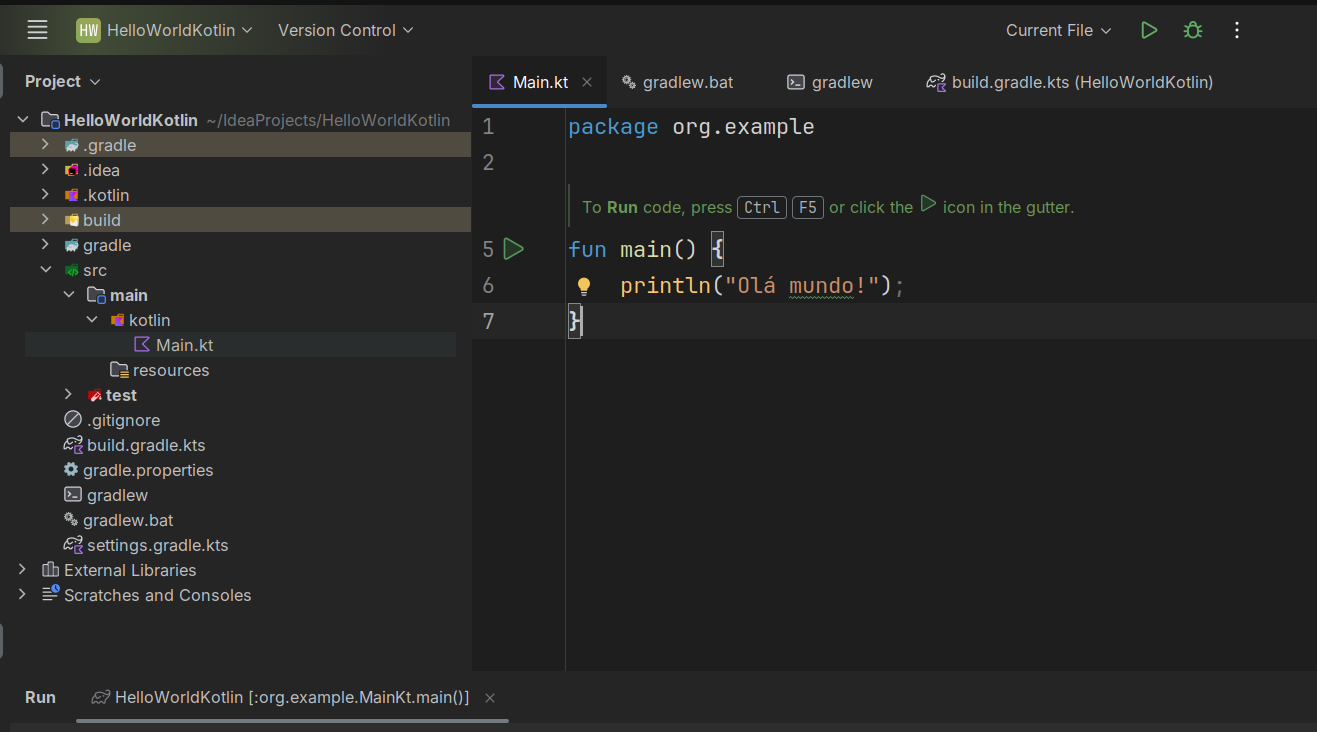
\includegraphics[width=\textwidth]{images/Captura de tela de 2026-07-31 10-14-22.png}
    \end{column}
  \end{columns}
\end{frame}

% -----------------------------------------------
% Seção: Fundamentos da Linguagem
% -----------------------------------------------
\section{Fundamentos da Linguagem}

\subsection{Variáveis: val vs var}

\begin{frame}[fragile]{Declaração de Variáveis: \texttt{val} vs \texttt{var}}
  \begin{columns}[T]
    \begin{column}{0.48\textwidth}
      \begin{block}{\centering \texttt{val} (Imutável / Somente Leitura)}
        \vspace{0.2em}
        \begin{itemize}\small
          \item \textbf{Valor fixo}: Atribuído apenas \textbf{uma vez}.
          \item Semelhante ao \texttt{final} no Java ou \texttt{const} em JS.
          \item \textbf{Recomendado}: Use \texttt{val} por padrão para código mais seguro e previsível.
        \end{itemize}
      \end{block}
      
      \vspace{0.4em}
      
      \begin{block}{\centering \texttt{var} (Mutável)}
        \vspace{0.2em}
        \begin{itemize}\small
          \item \textbf{Valor reatribuível}: Pode ser alterado ao longo da execução.
          \item O tipo da variável continua fixo (estaticamente tipado).
        \end{itemize}
      \end{block}
    \end{column}

    \begin{column}{0.49\textwidth}
      \textbf{Exemplo Prático:}
      \vspace{0.2em}

\begin{lstlisting}[style=KotlinStyle]
fun main() {
    // Imutavel (val)
    val cpf = "123.456.789-00"
    // cpf = "987.654.321-99" // Erro de Compilacao!

    // Mutavel (var)
    var contador = 0
    contador = 1 // Permitido!
    contador += 5

    println("CPF: $cpf")
    println("Contador: $contador")
}
\end{lstlisting}
    \end{column}
  \end{columns}
\end{frame}

\subsection{Tipos de Dados e Null Safety}

% Slide 1: Tipos Numéricos
\begin{frame}[fragile]{Tipos de Dados: Numéricos}
  \begin{columns}[T]
    \begin{column}{0.45\textwidth}
      \textbf{Inteiros e Ponto Flutuante}
      \vspace{0.3em}
      \begin{itemize}\small
        \item \textbf{Byte} (8 bits), \textbf{Short} (16 bits)
        \item \textbf{Int} (32 bits) — Padrão para inteiros
        \item \textbf{Long} (64 bits) — Sufixo \texttt{L}
        \item \textbf{Float} (32 bits) — Sufixo \texttt{f} ou \texttt{F}
        \item \textbf{Double} (64 bits) — Padrão para decimais
      \end{itemize}
    \end{column}
    \begin{column}{0.52\textwidth}
\begin{lstlisting}[style=KotlinStyle]
fun main() {
    val idade: Int = 25
    val habitantes: Long = 214000000L
    val peso: Float = 70.5f
    val preco: Double = 199.99

    println("Idade: $idade")
    println("Habitantes: $habitantes")
    println("Peso: $peso | Preco: $preco")
}
\end{lstlisting}
    \end{column}
  \end{columns}
\end{frame}

% Slide 2: Booleans e Caracteres
\begin{frame}[fragile]{Tipos de Dados: Boolean e Char}
  \begin{columns}[T]
    \begin{column}{0.45\textwidth}
      \textbf{Booleanos e Caracteres}
      \vspace{0.3em}
      \begin{itemize}\small
        \item \textbf{Boolean}: Representa valores lógicos (\texttt{true} ou \texttt{false}).
        \item Suporta operadores lógicos: \texttt{\&\&}, \texttt{||}, \texttt{!}.
        \item \textbf{Char}: Representa um único caractere Unicode envolvido por aspas simples (\texttt{' '}).
      \end{itemize}
    \end{column}
    \begin{column}{0.52\textwidth}
\begin{lstlisting}[style=KotlinStyle]
fun main() {
    val ativo: Boolean = true
    val maiorDeIdade: Boolean = false
    
    val genero: Char = 'M'
    val simbolo: Char = 'A'

    println("Ativo: $ativo")
    println("Pode dirigir? ${ativo && maiorDeIdade}")
    println("Genero: $genero")
}
\end{lstlisting}
    \end{column}
  \end{columns}
\end{frame}

% Slide 3: Strings e String Templates
\begin{frame}[fragile]{Tipos de Dados: String e Templates}
  \begin{columns}[T]
    \begin{column}{0.45\textwidth}
      \textbf{Cadeias de Caracteres}
      \vspace{0.3em}
      \begin{itemize}\small
        \item \textbf{String}: Sequência de caracteres entre aspas duplas (\texttt{" "}).
        \item \textbf{String Templates}: Interpolação de variáveis usando \texttt{\$nome}.
        \item Expressões complexas podem ser avaliadas usando \texttt{\${expressao}}.
        \item Suporta Strings de múltiplas linhas com três aspas (\texttt{""" """}).
      \end{itemize}
    \end{column}
    \begin{column}{0.52\textwidth}
\begin{lstlisting}[style=KotlinStyle]
fun main() {
    val nome = "Sergio"
    val sobrenome = "Novak"
    
    // String Template
    val nomeCompleto = "$nome $sobrenome"
    val mensagem = "Tamanho: ${nomeCompleto.length}"

    println(nomeCompleto)
    println(mensagem)
}
\end{lstlisting}
    \end{column}
  \end{columns}
\end{frame}

% Slide 4: Tipos Anuláveis (Nullable Types)
\begin{frame}[fragile]{Tipos Anuláveis (Nullable Types)}
  \begin{columns}[T]
    \begin{column}{0.45\textwidth}
      \textbf{Null Safety no Sistema de Tipos}
      \vspace{0.3em}
      \begin{itemize}\small
        \item Por padrão, os tipos em Kotlin \textbf{não aceitam nulo}.
        \item Adiciona-se o operador \texttt{?} para permitir valores nulos (\texttt{Tipo?}).
        \item Chamada segura: operador \texttt{?.}
        \item Operador Elvis: \texttt{?:} para fornecer um valor padrão.
      \end{itemize}
    \end{column}
    \begin{column}{0.52\textwidth}
\begin{lstlisting}[style=KotlinStyle]
fun main() {
    var apelido: String? = null
    
    // Chamada segura (retorna null se for null)
    println(apelido?.length)

    // Operador Elvis (retorna valor padrao)
    val exibicao = apelido ?: "Sem apelido"
    println(exibicao)
}
\end{lstlisting}
    \end{column}
  \end{columns}
\end{frame}

% -----------------------------------------------
% Seção: Funções em Kotlin
% -----------------------------------------------
\section{Funções em Kotlin}

\subsection{Declaração de Funções}

\begin{frame}[fragile]{Declaração de Funções}
  \begin{columns}[T]
    \begin{column}{0.46\textwidth}
      \textbf{Formas de Declarar Funções}
      \vspace{0.3em}
      \begin{itemize}\small
        \item \textbf{Funções de Expressão Única}:
          \begin{itemize}\footnotesize
            \item Sintaxe concisa usando o operador \texttt{=}.
            \item Opcional especificar o tipo de retorno quando o compilador infere.
          \end{itemize}
        \item \textbf{Funções com Corpo em Bloco}:
          \begin{itemize}\footnotesize
            \item Usam chaves \texttt{\{ \}} e exigem o comando \texttt{return} (se houver retorno).
            \item Requerem definição explícita do tipo de retorno.
          \end{itemize}
      \end{itemize}
    \end{column}
    \begin{column}{0.51\textwidth}
\begin{lstlisting}[style=KotlinStyle]
// Expressao de linha unica (Single-expression)
fun helloWorld(nome: String) = 
    println("Ola, $nome!")

// Corpo em bloco com retorno explicito
fun media(n1: Int, n2: Int): Int {
    val media = (n1 + n2) / 2
    return media
}

fun main() {
    helloWorld("sergio")
    println(media(10, 8))
}
\end{lstlisting}
    \end{column}
  \end{columns}
\end{frame}

\subsection{Expressões Lambda e Sintaxe}

% Slide 2: Funções Lambda e Comparativo com JS
\begin{frame}[fragile]{Funções Lambda (Sintaxe com Chaves \{\})}
  \begin{columns}[T]
    \begin{column}{0.46\textwidth}
      \textbf{Expressões Lambda em Kotlin}
      \vspace{0.3em}
      \begin{itemize}\small
        \item Forma comum de escrever \textit{arrow functions}.
        \item Toda a expressão fica contida dentro de chaves \texttt{\{ \}}.
        \item Usa a seta simples \texttt{->} para separar parâmetros do corpo (em vez de \texttt{=>}).
      \end{itemize}
    \end{column}
    \begin{column}{0.51\textwidth}
      \textbf{Comparativo: JavaScript vs. Kotlin}
      \vspace{0.2em}
\begin{lstlisting}[style=JavaStyle]
// JavaScript
const soma = (a, b) => a + b;
\end{lstlisting}

\begin{lstlisting}[style=KotlinStyle]
// Kotlin
val soma = { a: Int, b: Int -> a + b }

fun main() {
    println(soma(5, 3)) // Saida: 8
}
\end{lstlisting}
    \end{column}
  \end{columns}
\end{frame}

% Slide 3: O parâmetro implícito 'it'
\begin{frame}[fragile]{O Parâmetro Implícito \texttt{it}}
  \begin{columns}[T]
    \begin{column}{0.46\textwidth}
      \textbf{Simplificação para Parâmetro Único}
      \vspace{0.3em}
      \begin{itemize}\small
        \item Se a função lambda receber apenas um parâmetro, você não precisa declarar a seta \texttt{->}.
        \item O Kotlin disponibiliza automaticamente o nome \texttt{it} para se referir a esse parâmetro.
        \item Torna o código muito mais legível em operações com coleções (ex: \texttt{map}, \texttt{filter}).
      \end{itemize}
    \end{column}
    \begin{column}{0.51\textwidth}
\begin{lstlisting}[style=KotlinStyle]
// Em vez de: { x: Int -> x * 2 }
val numeros = listOf(1, 2, 3)

// Usando o parametro implicito 'it':
val dobrados = numeros.map { it * 2 }

fun main() {
    println(dobrados) // [2, 4, 6]
}
\end{lstlisting}
    \end{column}
  \end{columns}
\end{frame}

% Slide 4: Funções de Expressão Única (Single-Expression Functions)
\begin{frame}[fragile]{Funções de Expressão Única (Single-Expression)}
  \begin{columns}[T]
    \begin{column}{0.46\textwidth}
      \textbf{Funções de Linha Única com \texttt{=}}
      \vspace{0.3em}
      \begin{itemize}\small
        \item Declaradas com a palavra-chave \texttt{fun}.
        \item Quando possuem apenas uma linha de retorno, omite-se o bloco \texttt{\{ \}} e a palavra \texttt{return}.
        \item Utiliza-se apenas o operador \texttt{=}.
        \item O tipo de retorno é inferido automaticamente pelo compilador.
      \end{itemize}
    \end{column}
    \begin{column}{0.51\textwidth}
\begin{lstlisting}[style=KotlinStyle]
// Funcao tradicional
fun helloTradicional(nome: String): Unit {
    println("Ola, $nome!")
}

// Estilo de expressao unica
fun helloWorld(nome: String) = 
    println("Ola, $nome!")

// Exemplo com retorno de valor
fun dobro(n: Int) = n * 2
\end{lstlisting}
    \end{column}
  \end{columns}
\end{frame}

% Slide 5: Resumo das Diferenças de Sintaxe
\begin{frame}{Resumo das Diferenças de Sintaxe}
  \vspace{0.5em}
  \centering
  \begin{table}
    \small
    \begin{tabular}{l l l}
      \toprule
      \textbf{Conceito} & \textbf{JavaScript} & \textbf{Kotlin} \\
      \midrule
      \textbf{Seta utilizada} & \texttt{=>} & \texttt{->} \\[4pt]
      \textbf{Escopo da Lambda} & \texttt{(a, b) => a + b} & \texttt{\{ a, b -> a + b \}} \\[4pt]
      \textbf{Parâmetro único} & \texttt{x => x * 2} & \texttt{\{ it * 2 \}} \\[4pt]
      \textbf{Expressão única em função} & \textit{Não possui suporte nativo} & \texttt{fun dobro(n) = n * 2} \\
      \bottomrule
    \end{tabular}
  \end{table}
\end{frame}

% -----------------------------------------------
% Seção: Programação Orientada a Objetos em Kotlin
% -----------------------------------------------
\section{Orientação a Objetos em Kotlin}

\subsection{Classes, Objetos e Membros}

% Slide 5: Classes
\begin{frame}[fragile]{Classes em Kotlin}
  \begin{columns}[T]
    \begin{column}{0.46\textwidth}
      \textbf{O que é uma Classe?}
      \vspace{0.3em}
      \begin{itemize}\small
        \item Uma classe é um \textbf{modelo ou molde} para criação de objetos.
        \item Ela ainda \textbf{não ocupa memória} por si só.
        \item Apenas define a estrutura e comportamento que os objetos terão.
      \end{itemize}
    \end{column}
    \begin{column}{0.51\textwidth}
      \textbf{Sintaxe Básica:}
      \vspace{0.2em}
\begin{lstlisting}[style=KotlinStyle]
class Pessoa {
    // Corpo da classe (opcional se vazia)
}
\end{lstlisting}
    \end{column}
  \end{columns}
\end{frame}

% Slide 6: Objetos
\begin{frame}[fragile]{Objetos}
  \begin{columns}[T]
    \begin{column}{0.46\textwidth}
      \textbf{Instanciando Objetos}
      \vspace{0.3em}
      \begin{itemize}\small
        \item Objetos são \textbf{instâncias reais} de uma classe.
        \item Alocam espaço na memória ao serem criados.
        \item Cada objeto possui sua própria identidade e estado.
        \item Em Kotlin, \textbf{não} se usa a palavra-chave \texttt{new}.
      \end{itemize}
    \end{column}
    \begin{column}{0.51\textwidth}
\begin{lstlisting}[style=KotlinStyle]
class Pessoa

fun main() {
    // Criando objetos (instancias)
    val p1 = Pessoa()
    val p2 = Pessoa()
    
    // p1 e p2 sao objetos distintos
}
\end{lstlisting}
    \end{column}
  \end{columns}
\end{frame}

% Slide 7: Atributos
\begin{frame}[fragile]{Atributos}
  \begin{columns}[T]
    \begin{column}{0.46\textwidth}
      \textbf{Características dos Objetos}
      \vspace{0.3em}
      \begin{itemize}\small
        \item Atributos (propriedades) armazenam os dados/estado do objeto.
        \item Declarados com \texttt{var} (mutáveis) ou \texttt{val} (imutáveis).
        \item Acessados e alterados via notação de ponto (\texttt{objeto.atributo}).
      \end{itemize}
    \end{column}
    \begin{column}{0.51\textwidth}
\begin{lstlisting}[style=KotlinStyle]
class Pessoa {
    var nome = ""
    var idade = 0
}

fun main() {
    val pessoa = Pessoa()

    pessoa.nome = "Maria"
    pessoa.idade = 20

    println("${pessoa.nome} tem ${pessoa.idade} anos")
}
\end{lstlisting}
    \end{column}
  \end{columns}
\end{frame}

% Slide 8: Métodos
\begin{frame}[fragile]{Métodos}
  \begin{columns}[T]
    \begin{column}{0.46\textwidth}
      \textbf{Comportamento dos Objetos}
      \vspace{0.3em}
      \begin{itemize}\small
        \item Métodos são funções declaradas dentro de uma classe.
        \item Representam as ações/comportamentos que os objetos podem realizar.
        \item Podem acessar diretamente as propriedades da classe.
      \end{itemize}
    \end{column}
    \begin{column}{0.51\textwidth}
\begin{lstlisting}[style=KotlinStyle]
class Pessoa {
    var nome = ""

    fun apresentar() {
        println("Ola, meu nome e $nome")
    }
}

fun main() {
    val p = Pessoa()
    p.nome = "Carlos"
    p.apresentar()
}
\end{lstlisting}
    \end{column}
  \end{columns}
\end{frame}

\subsection{Construtores e Inicialização}

% Slide 9: Construtor Primário
\begin{frame}[fragile]{Construtor Primário}
  \begin{columns}[T]
    \begin{column}{0.46\textwidth}
      \textbf{Sintaxe Enxuta em Kotlin}
      \vspace{0.3em}
      \begin{itemize}\small
        \item O construtor primário faz parte do cabeçalho da classe.
        \item Declara e inicializa propriedades diretamente no parâmetro.
        \item Reduz significativamente o código boilerplate.
      \end{itemize}
    \end{column}
    \begin{column}{0.51\textwidth}
\begin{lstlisting}[style=KotlinStyle]
// Declaracao concisa com construtor primario
class Pessoa(
    var nome: String,
    var idade: Int
)

fun main() {
    // Instanciando e inicializando direto:
    val p = Pessoa("Ana", 22)
    println("${p.nome}, ${p.idade} anos")
}
\end{lstlisting}
    \end{column}
  \end{columns}
\end{frame}

% Slide 10: Construtores Secundários
\begin{frame}[fragile]{Construtores Secundários}
  \begin{columns}[T]
    \begin{column}{0.46\textwidth}
      \textbf{Múltiplas Formas de Construção}
      \vspace{0.3em}
      \begin{itemize}\small
        \item Declarados com a palavra \texttt{constructor}.
        \item Permitem fornecer construtores alternativos (ex: sem parâmetros e com parâmetros).
        \item Usam a referência \texttt{this} para atribuir aos atributos.
      \end{itemize}
    \end{column}
    \begin{column}{0.51\textwidth}
\begin{lstlisting}[style=KotlinStyle]
class Pessoa {
    var nome = ""
    var idade = 0

    constructor()

    constructor(nome: String, idade: Int) {
        this.nome = nome
        this.idade = idade
    }
}
\end{lstlisting}
    \end{column}
  \end{columns}
\end{frame}

% Slide 11: Inicialização (init)
\begin{frame}[fragile]{Inicialização com o bloco \texttt{init}}
  \begin{columns}[T]
    \begin{column}{0.46\textwidth}
      \textbf{Execução Automática}
      \vspace{0.3em}
      \begin{itemize}\small
        \item O bloco \texttt{init} é executado automaticamente assim que o objeto é instanciado.
        \item Útil para validações, logs ou inicializações complexas no construtor primário.
      \end{itemize}
    \end{column}
    \begin{column}{0.51\textwidth}
\begin{lstlisting}[style=KotlinStyle]
class Pessoa(
    var nome: String,
    var idade: Int
) {
    init {
        println("Objeto $nome criado com sucesso!")
    }
}

fun main() {
    val p = Pessoa("Lucas", 30)
}
\end{lstlisting}
    \end{column}
  \end{columns}
\end{frame}

\subsection{Encapsulamento e Visibilidade}

% Slide: Modificadores de Visibilidade - public
\begin{frame}[fragile]{Modificadores de Visibilidade: \texttt{public}}
  \begin{columns}[T]
    \begin{column}{0.46\textwidth}
      \textbf{Modificador Padrão}
      \vspace{0.3em}
      \begin{itemize}\small
        \item É o modificador de acesso padrão em Kotlin.
        \item Mesmo que você não escreva a palavra \texttt{public}, ela é assumida pelo compilador.
        \item Elementos públicos podem ser acessados de qualquer lugar.
      \end{itemize}
    \end{column}
    \begin{column}{0.51\textwidth}
      \textbf{Exemplos Equivalentes:}
\begin{lstlisting}[style=KotlinStyle]
class Pessoa {
    public var nome = "Maria"

    fun apresentar() {
        println(nome)
    }
}

// Equivalente a:
class Pessoa {
    var nome = "Maria"

    fun apresentar() {
        println(nome)
    }
}
\end{lstlisting}
    \end{column}
  \end{columns}
\end{frame}

% Slide: Modificadores de Visibilidade - private
\begin{frame}[fragile]{Modificadores de Visibilidade: \texttt{private}}
  \begin{columns}[T]
    \begin{column}{0.46\textwidth}
      \textbf{Restrição ao Escopo Local}
      \vspace{0.3em}
      \begin{itemize}\small
        \item Restringe o acesso estritamente ao próprio arquivo ou classe onde foi declarado.
        \item Impede que arquivos ou classes externas modifiquem ou leiam o atributo diretamente.
        \item Tentativas de acesso externo geram erro de compilação.
      \end{itemize}
    \end{column}
    \begin{column}{0.51\textwidth}
\begin{lstlisting}[style=KotlinStyle]
class ContaBancaria {
    private var saldo = 1000.0

    fun consultarSaldo() {
        println(saldo)
    }
}

fun main() {
    val conta = ContaBancaria()
    // Erro de Compilacao!
    // println(conta.saldo)
}
\end{lstlisting}
    \end{column}
  \end{columns}
\end{frame}

% Slide: Modificadores de Visibilidade - protected
\begin{frame}[fragile]{Modificadores de Visibilidade: \texttt{protected}}
  \begin{columns}[T]
    \begin{column}{0.46\textwidth}
      \textbf{Acesso por Subclasses}
      \vspace{0.3em}
      \begin{itemize}\small
        \item Só pode ser acessado pela própria classe e por suas subclasses (classes que a herdam).
        \item \textbf{Não é acessível} de forma externa através da instância da subclasse.
      \end{itemize}
    \end{column}
    \begin{column}{0.51\textwidth}
\begin{lstlisting}[style=KotlinStyle]
open class Animal {
    protected var energia = 100
}

class Cachorro : Animal() {
    fun brincar() {
        energia -= 10 // Permitido!
    }
}

fun main() {
    val c = Cachorro()
    // c.energia // Erro de Compilacao!
}
\end{lstlisting}
    \end{column}
  \end{columns}
\end{frame}

% Slide: Modificadores de Visibilidade - internal
\begin{frame}[fragile]{Modificadores de Visibilidade: \texttt{internal}}
  \begin{columns}[T]
    \begin{column}{0.46\textwidth}
      \textbf{Visibilidade no Mesmo Módulo}
      \vspace{0.3em}
      \begin{itemize}\small
        \item Modificador exclusivo da linguagem Kotlin.
        \item Permite acesso apenas dentro do \textbf{mesmo módulo} de compilação (ex: mesmo projeto Gradle ou módulo IntelliJ).
        \item Se a classe estiver em uma biblioteca, outro projeto que usar essa biblioteca não poderá acessá-la.
      \end{itemize}
    \end{column}
    \begin{column}{0.51\textwidth}
\begin{lstlisting}[style=KotlinStyle]
internal class BancoDados {
    fun conectar() {
        println("Conectado")
    }
}

// Visivel em todo o modulo atual,
// porem oculto para outros modulos/projetos.
\end{lstlisting}
    \end{column}
  \end{columns}
\end{frame}

% Slide: Tabela Comparativa de Visibilidade
\begin{frame}[fragile]{Comparativo de Visibilidade}
  \begin{columns}[T]
    \begin{column}{0.30\textwidth}
\begin{lstlisting}[style=KotlinStyle]
open class Pessoa {
    public var nome = "Ana"
    private var cpf = "123456"
    protected var idade = 20
    internal var univ = "UniRV"
}
\end{lstlisting}
    \end{column}
    \begin{column}{0.70\textwidth}
        \scriptsize

      \vspace{-0.5em}
      \begin{table}
        \scriptsize
        \begin{tabular}{l c c c c}
          \toprule
          \textbf{Membro} & \textbf{Mesma classe} & \textbf{Subclasse} & \textbf{Mesmo módulo} & \textbf{Outro módulo} \\
          \midrule
          \texttt{public}    & Sim & Sim & Sim & Sim \\[3pt]
          \texttt{private}   & Sim & N\~ao & N\~ao & N\~ao \\[3pt]
          \texttt{protected} & Sim & Sim & N\~ao & N\~ao \\[3pt]
          \texttt{internal}  & Sim & Sim & Sim & N\~ao \\
          \bottomrule
        \end{tabular}
      \end{table}
    \end{column}
  \end{columns}
\end{frame}

% Slide: Observação sobre Java e package-private
\begin{frame}{Diferença Importante em Relação ao Java}
  \begin{block}{Atenção: Ausência de \texttt{package-private}}
    \vspace{0.3em}
    Diferentemente de linguagens como Java, o Kotlin \textbf{não possui} o modificador de acesso \textit{package-private} (visibilidade restrita ao mesmo pacote).
    \vspace{0.5em}

    Em Kotlin, o equivalente mais próximo para compartilhar código dentro de um projeto é o modificador \textbf{\texttt{internal}}, cuja visibilidade é baseada no \textbf{módulo} (compilação), e não no pacote.
  \end{block}
\end{frame}

% Slide 13: Getters e Setters
\begin{frame}[fragile]{Getters e Setters}
  \begin{columns}[T]
    \begin{column}{0.46\textwidth}
      \textbf{Acesso e Validação de Propriedades}
      \vspace{0.3em}
      \begin{itemize}\small
        \item Kotlin gera automaticamente getters e setters padrão.
        \item É possível personalizá-los diretamente abaixo da propriedade.
        \item Usa-se \texttt{field} (field de apoio) dentro do getter/setter para evitar recursão infinita.
      \end{itemize}
    \end{column}
    \begin{column}{0.51\textwidth}
\begin{lstlisting}[style=KotlinStyle]
class Pessoa {
    var idade = 0
        set(value) {
            if (value >= 0) {
                field = value
            }
        }
}

fun main() {
    val p = Pessoa()
    p.idade = -5 // Nao altera
    println(p.idade) // Saida: 0
}
\end{lstlisting}
    \end{column}
  \end{columns}
\end{frame}

\subsection{Herança, Polimorfismo e Abstração}

% Slide 14: Herança
\begin{frame}[fragile]{Herança}
  \begin{columns}[T]
    \begin{column}{0.46\textwidth}
      \textbf{Reaproveitamento de Código}
      \vspace{0.3em}
      \begin{itemize}\small
        \item Em Kotlin, todas as classes são \texttt{final} por padrão (não podem ser herdadas).
        \item Deve-se usar a palavra-chave \texttt{open} para permitir herança.
        \item A sintaxe de herança usa dois pontos (\texttt{: SuperClasse()}).
      \end{itemize}
    \end{column}
    \begin{column}{0.51\textwidth}
\begin{lstlisting}[style=KotlinStyle]
// Classe base aberta para heranca
open class Animal {
    fun dormir() {
        println("Dormindo...")
    }
}

// Classe filha herdando de Animal
class Cachorro : Animal()
\end{lstlisting}
    \end{column}
  \end{columns}
\end{frame}

% Slide 15: Sobrescrita (override)
\begin{frame}[fragile]{Sobrescrita de Métodos (\texttt{override})}
  \begin{columns}[T]
    \begin{column}{0.46\textwidth}
      \textbf{Redefinindo Comportamentos}
      \vspace{0.3em}
      \begin{itemize}\small
        \item O método da classe pai também precisa ser marcado com \texttt{open}.
        \item A classe filha usa a palavra-chave \texttt{override} para redefinir a implementação.
      \end{itemize}
    \end{column}
    \begin{column}{0.51\textwidth}
\begin{lstlisting}[style=KotlinStyle]
open class Animal {
    open fun emitirSom() {
        println("Som generico")
    }
}

class Cachorro : Animal() {
    override fun emitirSom() {
        println("Au Au")
    }
}
\end{lstlisting}
    \end{column}
  \end{columns}
\end{frame}

% Slide 16: Polimorfismo
\begin{frame}[fragile]{Polimorfismo}
  \begin{columns}[T]
    \begin{column}{0.46\textwidth}
      \textbf{Múltiplas Formas}
      \vspace{0.3em}
      \begin{itemize}\small
        \item Permite tratar objetos de classes filhas como se fossem do tipo da classe pai.
        \item O método executado é o da classe instanciada em tempo de execução.
        \item \textit{Mesmo tipo genérico produzindo comportamentos diferentes.}
      \end{itemize}
    \end{column}
    \begin{column}{0.51\textwidth}
\begin{lstlisting}[style=KotlinStyle]
fun main() {
    // Tipo da superclasse, instancia da filha
    val animal: Animal = Cachorro()

    animal.emitirSom() 
    // Resultado: "Au Au"
}
\end{lstlisting}
    \end{column}
  \end{columns}
\end{frame}

% Slide 17: Classes Abstratas
\begin{frame}[fragile]{Classes Abstratas}
  \begin{columns}[T]
    \begin{column}{0.46\textwidth}
      \textbf{Modelos Incompletos}
      \vspace{0.3em}
      \begin{itemize}\small
        \item Declaradas com \texttt{abstract}.
        \item Não podem ser instanciadas diretamente.
        \item Podem ter métodos abstratos (sem corpo) que obrigam a classe filha a implementar.
      \end{itemize}
    \end{column}
    \begin{column}{0.51\textwidth}
\begin{lstlisting}[style=KotlinStyle]
abstract class Forma {
    abstract fun desenhar()
}

class Circulo : Forma() {
    override fun desenhar() {
        println("Desenhando um circulo")
    }
}
\end{lstlisting}
    \end{column}
  \end{columns}
\end{frame}

% Slide 18: Interfaces
\begin{frame}[fragile]{Interfaces}
  \begin{columns}[T]
    \begin{column}{0.46\textwidth}
      \textbf{Contratos de Comportamento}
      \vspace{0.3em}
      \begin{itemize}\small
        \item Definem contratos de ações que uma classe deve cumprir.
        \item Uma classe pode implementar múltiplas interfaces.
        \item Métodos em interfaces são abstratos por padrão.
      \end{itemize}
    \end{column}
    \begin{column}{0.51\textwidth}
\begin{lstlisting}[style=KotlinStyle]
interface Voador {
    fun voar()
}

class Passaro : Voador {
    override fun voar() {
        println("Voando...")
    }
}
\end{lstlisting}
    \end{column}
  \end{columns}
\end{frame}

% Slide 19: Herança vs. Interface
\begin{frame}{Comparativo: Herança $\times$ Interface}
  \vspace{0.5em}
  \centering
  \begin{table}
    \scriptsize
    \begin{tabular}{l l l}
      \toprule
      \textbf{Característica} & \textbf{Herança} & \textbf{Interface} \\
      \midrule
      \textbf{Relacionamento} & "É um" (ex: Cachorro \textit{é um} Animal) & "Pode fazer" (ex: Passaro \textit{pode} Voar) \\[4pt]
      \textbf{Quantidade} & Apenas uma superclasse & Múltiplas interfaces \\[4pt]
      \textbf{Propósito} & Compartilha código/implementação & Compartilha contrato de comportamento \\
      \bottomrule
    \end{tabular}
  \end{table}
\end{frame}

% Slide 20: Exemplo Completo
\begin{frame}[fragile]{Exemplo Completo de Orientação a Objetos}
  \begin{columns}[T]
    \begin{column}{0.46\textwidth}
      \textbf{Hierarquia de Funcionários}
      \vspace{0.3em}
      \begin{itemize}\small
        \item Superclasse \texttt{Funcionario} aberta.
        \item Subclasse \texttt{Professor} sobrescrevendo a lógica de salário baseada nas horas.
        \item Integração de Construtores, Herança e Sobrescrita.
      \end{itemize}
    \end{column}
    \begin{column}{0.51\textwidth}
\begin{lstlisting}[style=KotlinStyle]
open class Funcionario(var nome: String) {
    open fun salario(): Double = 0.0
}

class Professor(
    nome: String,
    var horas: Int
) : Funcionario(nome) {
    override fun salario(): Double {
        return horas * 80.0
    }
}

fun main() {
    val prof = Professor("Joao", 40)
    println(prof.salario()) // 3200.0
}
\end{lstlisting}
    \end{column}
  \end{columns}
\end{frame}

\subsection{Membros Estáticos (companion object)}

% Slide 21: Atributos e Métodos Estáticos (companion object)
\begin{frame}[fragile]{Membros Estáticos (\texttt{companion object})}
  \begin{columns}[T]
    \begin{column}{0.46\textwidth}
      \textbf{Membros de Classe em Kotlin}
      \vspace{0.3em}
      \begin{itemize}\small
        \item Kotlin não possui a palavra-chave \texttt{static}.
        \item Em seu lugar, utiliza-se o bloco \texttt{companion object} dentro da classe.
        \item Permite acessar atributos e métodos diretamente pela classe, sem precisar instanciá-la.
        \item Útil para constantes globais, métodos utilitários e padrão \textit{Factory}.
      \end{itemize}
    \end{column}
    \begin{column}{0.51\textwidth}
\begin{lstlisting}[style=KotlinStyle]
class Matematica {
    companion object {
        // Atributo "estatico"
        val PI = 3.14159

        // Metodo "estatico"
        fun dobro(n: Int): Int {
            return n * 2
        }
    }
}

fun main() {
    // Acesso direto pela classe:
    println(Matematica.PI)
    println(Matematica.dobro(5)) // 10
}
\end{lstlisting}
    \end{column}
  \end{columns}
\end{frame}

% -----------------------------------------------
% Seção: Recursos Adicionais para a Lista de Exercícios
% -----------------------------------------------
\section{Entrada de Dados, Vetores, Matrizes e Matemática}

\subsection{Leitura de Dados do Terminal (Escaneamento)}

% Slide: Leitura do Terminal com readln() e Scanner
\begin{frame}[fragile]{Leitura do Terminal em Kotlin}
  \begin{columns}[T]
    \begin{column}{0.46\textwidth}
      \textbf{Lendo Dados do Usuário}
      \vspace{0.3em}
      \begin{itemize}\small
        \item \textbf{\texttt{readln()}}: Função nativa e moderna do Kotlin (substituiu o antigo \texttt{readLine()!!}).
        \item Retorna sempre uma \texttt{String}.
        \item É necessário converter o tipo retornado usando métodos como \texttt{.toInt()}, \texttt{.toDouble()}, etc.
        \item Também é possível usar a classe \textbf{\texttt{Scanner}} da biblioteca Java (\texttt{java.util.Scanner}).
      \end{itemize}
    \end{column}
    \begin{column}{0.51\textwidth}
\begin{lstlisting}[style=KotlinStyle]
import java.util.Scanner

fun main() {
    // 1. Usando a funcao nativa readln()
    print("Digite seu nome: ")
    val nome = readln()

    print("Digite sua idade: ")
    val idade = readln().toInt()

    print("Digite sua nota: ")
    val nota = readln().toDouble()

    // 2. Usando a classe Scanner do Java
    val scanner = Scanner(System.`in`)
    print("Digite o peso: ")
    val peso = scanner.nextDouble()

    println("Nome: $nome | Idade: $idade")
}
\end{lstlisting}
    \end{column}
  \end{columns}
\end{frame}

\subsection{Vetores (Arrays) e Coleções}

% Slide: Vetores / Arrays em Kotlin
\begin{frame}[fragile]{Vetores (Arrays) em Kotlin}
  \begin{columns}[T]
    \begin{column}{0.46\textwidth}
      \textbf{Manipulação de Vetores}
      \vspace{0.3em}
      \begin{itemize}\small
        \item Criados com \texttt{arrayOf(...)} ou tipos primitivos dedicados como \texttt{IntArray}, \texttt{DoubleArray}.
        \item Acesso por índice via colchetes: \texttt{vetor[0]}.
        \item Propriedades e funções úteis: \texttt{.size}, \texttt{.sort()}, \texttt{.forEach \{ \}}.
      \end{itemize}
    \end{column}
    \begin{column}{0.51\textwidth}
\begin{lstlisting}[style=KotlinStyle]
fun main() {
    // Vetor de inteiros
    val numeros = intArrayOf(50, 10, 30, 20, 40)

    // Acessando e alterando valores
    println("Primeiro: ${numeros[0]}")
    numeros[0] = 99

    // Ordenacao de vetor
    numeros.sort()

    // Percorrendo o vetor
    for (n in numeros) {
        print("$n ")
    }
}
\end{lstlisting}
    \end{column}
  \end{columns}
\end{frame}

\subsection{Matrizes (Arrays Multidimensionais)}

% Slide: Matrizes em Kotlin
\begin{frame}[fragile,shrink=5]{Matrizes em Kotlin}
  \begin{columns}[T]
    \begin{column}{0.46\textwidth}
      \textbf{Matrizes (Arrays 2D)}
      \vspace{0.3em}
      \begin{itemize}\small
        \item Uma matriz é um vetor de vetores: \texttt{Array<Array<Tipo>>}.
        \item Acesso por dois índices: \texttt{matriz[linha][coluna]}.
        \item Inicializadas com \texttt{Array(linhas) \{ Array(colunas) \{ valor \} \}} ou listas de vetores.
      \end{itemize}
    \end{column}
    \begin{column}{0.51\textwidth}
\begin{lstlisting}[style=KotlinStyle]
fun main() {
    // Criando uma matriz 2x3 de Ints
    val matriz = arrayOf(
        intArrayOf(1, 2, 3),
        intArrayOf(4, 5, 6)
    )

    // Acessando elemento (linha 1, coluna 2)
    println("Valor [1][2]: ${matriz[1][2]}") // 6

    // Percorrendo a matriz com for aninhado
    for (i in matriz.indices) {
        for (j in matriz[i].indices) {
            print("${matriz[i][j]} ")
        }
        println()
    }
}
\end{lstlisting}
    \end{column}
  \end{columns}
\end{frame}

\subsection{Funções Matemáticas: Seno, Cosseno e Pacote kotlin.math}

% Slide: Seno, Cosseno e kotlin.math
\begin{frame}[fragile]{Funções Matemáticas: Seno e Cosseno}
  \begin{columns}[T]
    \begin{column}{0.46\textwidth}
      \textbf{Trigonometria com \texttt{kotlin.math}}
      \vspace{0.3em}
      \begin{itemize}\small
        \item Importe as funções do pacote \texttt{kotlin.math.*}.
        \item \textbf{\texttt{sin(x)}} e \textbf{\texttt{cos(x)}} recebem o ângulo obrigatoriamente em \textbf{radianos}.
        \item Use \textbf{\texttt{Math.toRadians(graus)}} para converter graus para radianos.
        \item Outras constantes úteis: \texttt{PI}, \texttt{sqrt()}, \texttt{pow()}, \texttt{abs()}.
      \end{itemize}
    \end{column}
    \begin{column}{0.51\textwidth}
\begin{lstlisting}[style=KotlinStyle]
import kotlin.math.sin
import kotlin.math.cos
import kotlin.math.PI

fun main() {
    val anguloGraus = 90.0
    // Converter graus para radianos
    val anguloRadianos = Math.toRadians(anguloGraus)

    val seno = sin(anguloRadianos)
    val cosseno = cos(anguloRadianos)

    println("Seno de 90 deg: $seno")       // 1.0
    println("Cosseno de 90 deg: $cosseno") // ~0.0
    println("Valor de PI: $PI")
}
\end{lstlisting}
    \end{column}
  \end{columns}
\end{frame}

\subsection{Coleções em Kotlin (Lists, Sets, Maps)}

% Slide 1: Coleções Imutáveis vs Mutáveis
\begin{frame}[fragile]{Coleções em Kotlin: Imutáveis vs Mutáveis}
  \begin{columns}[T]
    \begin{column}{0.46\textwidth}
      \textbf{Visão Geral de Coleções}
      \vspace{0.3em}
      \begin{itemize}\small
        \item Kotlin diferencia estritamente coleções \textbf{imutáveis} (somente leitura) de \textbf{mutáveis} (alteráveis).
        \item \textbf{Imutáveis (Padrão)}: \texttt{listOf()}, \texttt{setOf()}, \texttt{mapOf()}.
        \item \textbf{Mutáveis}: \texttt{mutableListOf()}, \texttt{mutableSetOf()}, \texttt{mutableMapOf()}.
        \item Métodos para alteração: \texttt{.add()}, \texttt{.remove()}, \texttt{.clear()}.
      \end{itemize}
    \end{column}
    \begin{column}{0.51\textwidth}
\begin{lstlisting}[style=KotlinStyle]
fun main() {
    // Lista Imutavel (read-only)
    val frutas = listOf("Maca", "Banana", "Uva")
    // frutas.add("Laranja") // Erro de Compilacao!

    // Lista Mutavel
    val nomes = mutableListOf("Sergio", "Ana")
    nomes.add("Carlos") // Permitido!
    nomes.remove("Ana")

    println("Frutas: $frutas")
    println("Nomes: $nomes")
}
\end{lstlisting}
    \end{column}
  \end{columns}
\end{frame}

% Slide 2: List, Set e Map
\begin{frame}[fragile]{Tipos de Coleções: List, Set e Map}
  \begin{columns}[T]
    \begin{column}{0.46\textwidth}
      \textbf{List, Set e Map}
      \vspace{0.3em}
      \begin{itemize}\small
        \item \textbf{List}: Coleção ordenada com acesso por índice. Aceita elementos duplicados.
        \item \textbf{Set}: Coleção de elementos \textbf{únicos} (sem duplicatas). Ordem não garantida.
        \item \textbf{Map}: Par Chave-Valor (\texttt{chave to valor}). Chaves devem ser únicas.
      \end{itemize}
    \end{column}
    \begin{column}{0.51\textwidth}
\begin{lstlisting}[style=KotlinStyle]
fun main() {
    // Set (nao aceita duplicatas)
    val codigos = setOf(101, 102, 101, 103)
    println(codigos) // [101, 102, 103]

    // Map (par Chave -> Valor)
    val capitais = mapOf(
        "GO" to "Goiania",
        "SP" to "Sao Paulo",
        "DF" to "Brasilia"
    )
    println("Capital de GO: ${capitais["GO"]}")
}
\end{lstlisting}
    \end{column}
  \end{columns}
\end{frame}

% Slide: Comparativo Java vs Kotlin para Coleções
\begin{frame}{Equivalência de Coleções: Java $\times$ Kotlin}
  \vspace{0.3em}
  \centering
  \begin{table}
    \scriptsize
    \begin{tabular}{l l l}
      \toprule
      \textbf{Conceito / Tipo} & \textbf{Java (Orientado a Objetos)} & \textbf{Kotlin (Imutável / Mutável)} \\
      \midrule
      \textbf{Lista de Leitura} & \texttt{Collections.unmodifiableList(...)} & \texttt{listOf("A", "B")} (Leitura) \\[4pt]
      \textbf{Lista Mutável (ArrayList)} & \texttt{new ArrayList<String>()} & \texttt{mutableListOf()} ou \texttt{arrayListOf()} \\[4pt]
      \textbf{Conjunto (Set)} & \texttt{new HashSet<Integer>()} & \texttt{setOf()} ou \texttt{mutableSetOf()} \\[4pt]
      \textbf{Mapa (Map / HashMap)} & \texttt{new HashMap<String, String>()} & \texttt{mapOf("K" to "V")} ou \texttt{mutableMapOf()} \\
      \bottomrule
    \end{tabular}
  \end{table}
  \vspace{0.3em}
  {\tiny \textit{Nota: Por baixo dos panos (na JVM), o Kotlin reutiliza as próprias classes nativas do Java (\texttt{java.util.ArrayList}, \texttt{HashSet}, \texttt{HashMap}), porém aplicando a distinção entre interfaces mutáveis e imutáveis em tempo de compilação.}}
\end{frame}

% Slide: Código Comparativo Java vs Kotlin
\begin{frame}[fragile]{Sintaxe Lado a Lado: Java $\times$ Kotlin}
  \begin{columns}[T]
    \begin{column}{0.49\textwidth}
      {\footnotesize\textcolor{kotlinorange}{\textbf{Java (Verboso e Mutável)}}}
\begin{lstlisting}[style=JavaStyle]
import java.util.*;

// List / ArrayList
List<String> lista = new ArrayList<>();
lista.add("Item 1");

// Set / HashSet
Set<Integer> conjunto = new HashSet<>();
conjunto.add(10);

// Map / HashMap
Map<String, Integer> mapa = new HashMap<>();
mapa.put("Chave", 100);
\end{lstlisting}
    \end{column}

    \begin{column}{0.49\textwidth}
      {\footnotesize\textcolor{kotlinpurple}{\textbf{Kotlin (Conciso e Seguro)}}}
\begin{lstlisting}[style=KotlinStyle]
// ArrayList Mutavel
val lista = mutableListOf("Item 1")
val lista2 = arrayListOf("Item 1") // nativo

// Set (HashSet)
val conjunto = mutableSetOf(10)
val conjunto2 = hashSetOf(10)

// Map (HashMap)
val mapa = mutableMapOf("Chave" to 100)
val mapa2 = hashMapOf("Chave" to 100)
\end{lstlisting}
    \end{column}
  \end{columns}
\end{frame}

% Slide 3: Operações Funcionais em Coleções (filter, map, forEach)
\begin{frame}[fragile]{Operações Funcionais em Coleções}
  \begin{columns}[T]
    \begin{column}{0.46\textwidth}
      \textbf{Processamento Funcional}
      \vspace{0.3em}
      \begin{itemize}\small
        \item \textbf{\texttt{filter \{ \}}}: Filtra elementos por uma condição.
        \item \textbf{\texttt{map \{ \}}}: Transforma elementos de uma coleção.
        \item \textbf{\texttt{find \{ \}}}, \textbf{\texttt{first()}}, \textbf{\texttt{count()}}, \textbf{\texttt{sorted()}}.
        \item Usam lambdas e o parâmetro implícito \texttt{it}.
      \end{itemize}
    \end{column}
    \begin{column}{0.51\textwidth}
\begin{lstlisting}[style=KotlinStyle]
fun main() {
    val numeros = listOf(1, 2, 3, 4, 5, 6, 7, 8)

    // Filtrar apenas pares
    val pares = numeros.filter { it % 2 == 0 }

    // Mapear (dobrar valores)
    val dobrados = numeros.map { it * 2 }

    println("Pares: $pares")       // [2, 4, 6, 8]
    println("Dobrados: $dobrados") // [2, 4, 6, ..., 16]
}
\end{lstlisting}
    \end{column}
  \end{columns}
\end{frame}

\end{document}
